
\chapter{\uppercase{Introduction and Motivation}}
\label{introduction}

\section*{List of Symbols}
\begin{singlespace}
\printnomenclature
\end{singlespace}

Numerical simulations are extensively used in science and engineering research to solve real world problems whose theoretical solutions are undetermined and in cases where it is impractical to conduct experiments.
For example, analytical solution for the general Navier-Stokes equations is unknown and it is impractical to conduct experiments on vehicles operating in hostile and unpredictable environmental conditions 
(e.g. reentry vehicles).
Under such circumstances computational methods are very powerful in assisting the design process and they play a pivotal role in design improvements and reductions in development cost and time.


In recent years, owing to an increasing availability of computational resources and sophisticated algorithms, numerical methods have been extensively used in engineering research and development. However, in spite of several advancements in computer hardware (e.g. CPU speed) and the increasing use of parallel computing (also known as high performance computing), a striking imbalance still exists between the requirements and availability of computational power.
For example, the number of required mesh points for direct numerical simulations (DNS) scales with the Reynolds number as $Re^{9/4}$, but the current state-of-the-art computing can only support on the order of $10^{9}$ - $10^{10}$ mesh points and is thus limited to Reynolds numbers of about $10,000$.  Similarly, other high-fidelity physics-based simulations such as large eddy simulations (LES) and unsteady Reynolds-averaged Navier-Stokes (RANS) computations, also require significant amounts of computational resources and time.


A simple gradient-based airfoil shape optimization requires many optimizer iterations and hence flow solutions. The entire flow field needs to be solved for at each design iteration and typically the gradient also needs to be computed (through finite-difference, adjoint~\cite{Pironneau74,Jameson95,Errico97} or other techniques), which in total can require hundreds of flow solutions, potentially demanding enormous computational time and storage. 
Therefore, the designer has to trade-off accuracy versus computational time or limit the design spaces in scope, which can  lead to inefficient designs. 
Such a computational burden explains the need for alternatives to expensive high-fidelity simulations, at least when function evaluations are repeatedly required.


\section{Surrogate Models}
In order to reduce the computational burden from multiple simulations, surrogate models (also called response surfaces or metamodels) have been employed by the research community over the past few decades.
Surrogate models provide an ``approximate and inexpensive to evaluate'' representation of an output quantity of interest as a function of input variables.
A surrogate model, being an approximate representation of the original function space, is bound to have an approximation error.
A lot of today's surrogate model research is directed on improving the accuracy of existing models as well as developing versatile and robust surrogates~\cite{Wiener38,Xiu2003,Cressie90,Koehler96,Yamazaki2010} considering its wide range of applications. 
Some popular applications are discussed in the following paragraphs.

\subsection{Applications of Surrogate Models}

In general, a surrogate model is used to approximate or predict a quantity of interest based on available computational, experimental or statistical data, and hence finds applications in a wide array of disciplines.  Some popular engineering applications are reviewed as follows.

\subsubsection{Database of Expensive Functions}
In early stages of a design process it is desirable to rapidly evaluate several design configurations. These analyses, that can either be physical experiments or numerical simulations, are expensive and time-consuming.
As an example, in the design of aerospace systems one of the main requirements is the accurate and efficient prediction of force and moment coefficients of the vehicle. 
This information is required for different trial designs, and an optimization procedure requires many design iterations (trials), which can be very expensive and prolong the time span of the whole design process.
Moreover, design of complex systems such as airplanes are highly coupled with several disciplines (e.g. propulsion, aerodynamics, structures, controls, etc.) demanding many such optimization processes.
Due to these time-intensive operations, developing a successful design and its associated production can take a long development time.
%Thus it becomes a highly prohibitive practice to test prototypes to obtain necessary data for design 
%(e.g repeating wind tunnel tests or simulations to get lift coefficients of an airfoil) and perhaps also due to the difficulties involved with multiple testing and budget cuts.
Hence, design teams are shifting their focus on building databases that could aid in the design process. Some examples are:
\begin{itemize}
\item {NASA's \textit{Constellation program} has been working on a Heavy Lift Launch Vehicle (HLLV) named Ares V, 
where a simulation protocol was developed to generate databases of the aerodynamic force and moment coefficients for HLLV ascent~\cite{Kiris2011}.}
\item {The NASA Langley Research Center was involved in the development of a preflight aerodynamic database of the X-34 Reusable Launch Vehicle (RLV)~\cite{Freeman1996}, covering the entire range of Mach numbers, angles of attack, side-slip and control surface deflections anticipated in the complete flight envelope.}
\item{The Center for Computer Applications in Aerospace Science and Engineering (a part of DLR) is working towards a ``Digital Flight'' (full flight simulation), 
for which they develop databases covering the entire flight envelope for many different aircraft configurations.} %${C^2}{A^2}{S^2}{E}$,
\end{itemize}
For such applications, surrogate models can be employed to predict the exact function values, thereby providing a computational advantage through an effective reduction of the overall number of required exact simulations. 
%However, as the number of input variables increase, the number of required simulations to cover the entire design space increases dramatically making even surrogate-based approximations expensive.

\subsubsection{Global Optimization}
Gradient-based optimization algorithms typically converge to a local optimum and the final optimum is highly dependent on the starting point in the design space. 
There is no guarantee that the gradient-based optimizers lead to the global optimum unless the convexity of the objective function is guaranteed. 
An illustration of a multi-modal design space with several local optimum is provided in Figure~\ref{fig:GlobalOpt}.
On the other hand, global optimization strategies such as the genetic algorithms (GA), which are based on an extensive search of the design space, are computationally intensive particularly when applied to problems involving high-fidelity physics-based simulations. 
A surrogate model can be employed to alleviate some of the computational burden in this process. For example, when a surrogate model is constructed with the given training data, the most promising locations in the model can be explored for relatively lower computational cost. To aid in this, an initial global surrogate model is constructed using the available training data. The surrogate model is then sampled extensively to find the potential global optimum and the model is locally updated or refined until reaching the optimum.
\begin{figure}[h]
\centering
\begin{minipage}[b]{0.5\linewidth}
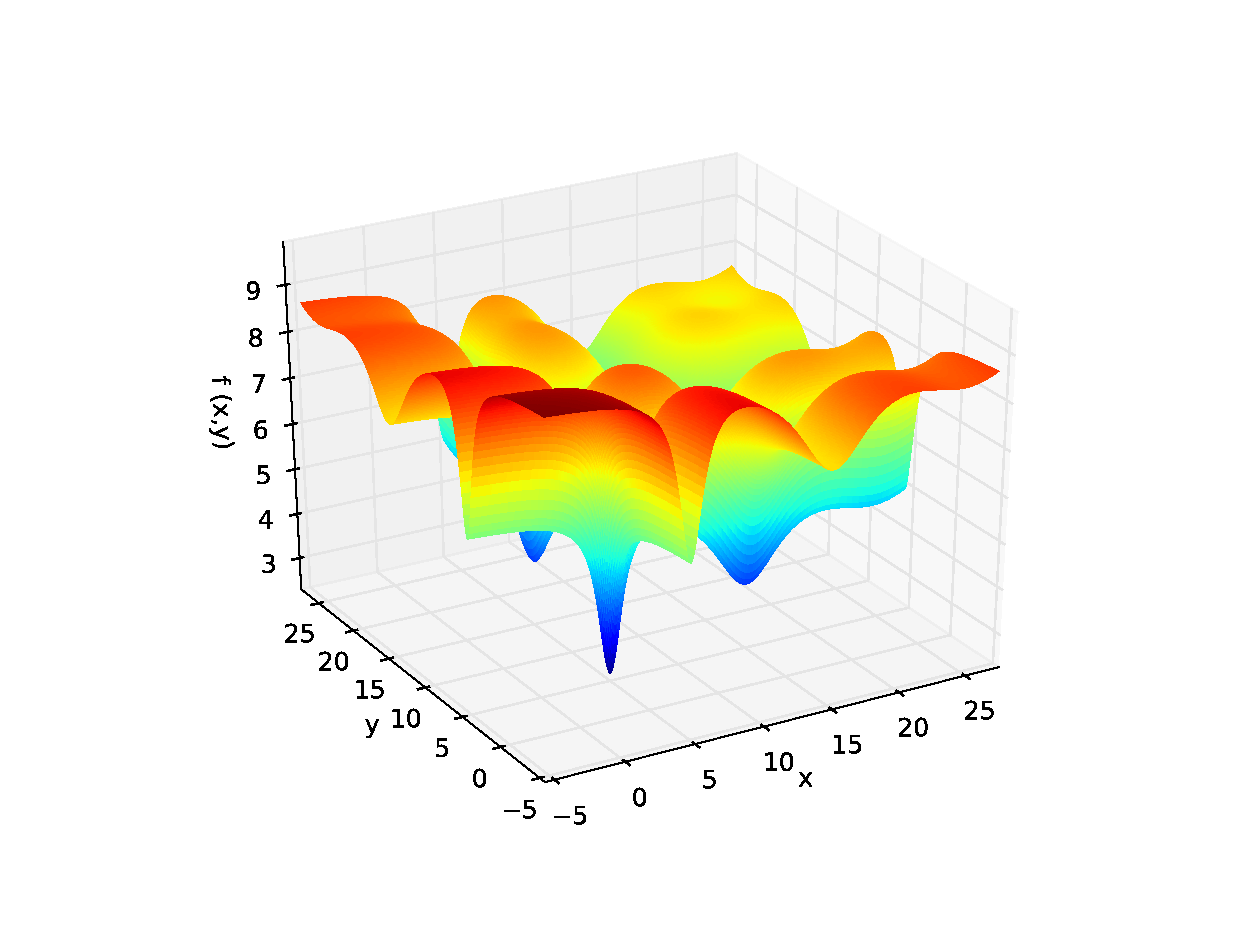
\includegraphics[width=1.0\textwidth]{GlobalOpt.eps}
\end{minipage}
\caption{A two variable multi-modal objective function.}
\label{fig:GlobalOpt}
\end{figure}
Even for such optimization applications, the construction of an accurate initial global surrogate model provokes a higher likelihood of locating the global optimum during subsequent local refinements of the surrogate model, when compared to a poor initial surrogate that fails to capture the real behavior leading to a premature convergence.

\subsubsection{Uncertainty Quantification and Optimization Under Uncertainty}

%To overcome this problem, a surrogate model (or response surface) can be built, using a limited number of simulation outputs $f(\z)$, which can then be inexpensively probed yielding approximated output function values $\hat{f}(\z)$.

A deterministic optimization approach assumes no variations in the design variables and other parameters. This can easily lead to sub-optimal performance or failure of many deterministically optimized designs. 
For instance, when an aircraft designed to cruise at specific optimal settings (e.g. Mach number, angle of attack, shape) deviates from these settings (e.g.~due to continuous  wind gusts, ice accumulation, faulty calibration of instruments, wear and tear) 
the flight performance can be adversely affected leading to an increased fuel burn or other undesirable characteristics.
Therefore, given the uncertainties in input variables, parameters and operating environments, it is expected to have some measure of confidence placed on the output quantities of interest (e.g. weight, thrust, lift etc.), 
giving rise to the field of uncertainty quantification (UQ) and optimization under uncertainty (OUU).
Optimization under uncertainty (also known as stochastic optimization) is an important avenue in computational research owing to the rising need for robust and reliable designs, where the key objective is to quantify uncertainties and account for them in the regular optimization process. 
OUU can be subdivided into two main fields namely: \emph{robust design optimization} (RDO) and \emph{reliability based design optimization} (RBDO)~\cite{Arora2007,Agarwal2004,Padmanaban2003}.
RDO techniques can be used to produce a design that is more robust (less sensitive) to design variable and/or operating environment changes, whereas RBDO minimizes the probability of failure of the system. 

In recent years, design teams and regulatory agencies are increasingly being asked to specifically characterize and quantify different types of uncertainties and separate their individual effects~\cite{Sandia2000,Sandia2006,Sandia2006b,Sandia2007,Sandia2008}.
The most popular and easiest approach for the propagation of uncertainties is the Monte Carlo simulation (MCS), where the simulation output $f$ is sampled many times to obtain output statistics and to determine worst case scenarios.
However, multiple realizations of the output function $f$ are not always computationally tractable (e.g. for high-fidelity physics-based simulations such as computational fluid dynamics (CFD) or finite element analyses (FEA)).
To overcome this problem, a surrogate model can be constructed to model the uncertainties, which can then be sampled inexpensively and exhaustively to propagate the uncertainties and determine output statistics.
This approach is referred to as the inexpensive Monte Carlo simulation (IMCS)~\cite{Ghate2006}. More details on these topics are provided in chapter~\ref{OUUFramework}.



%This paper deals with robust designs of systems taking into account the uncertainties in input variables and operating conditions.


%\subsubsection*{Uncertainty Quantification}

\subsection{Research Avenues}
\label{methodology}
Major research  areas which are extensively pursued related to surrogate modeling are discussed in the following paragraphs.


\subsubsection{Choice of Training Points}\label{choiceoftrainingpoints}
The accuracy of a surrogate model is influenced primarily by the non-linearity of the function to be modeled and by the choice of training point locations.
Training point selection is typically done by using design of experiments (DoE) techniques such as uniform design (UD)~\cite{Fang2000}.
Many other methods, which have been originally developed to approximate multi-dimensional integrals, are also being used for training data selection for surrogate models: these include Monte Carlo (MC)~\cite{Metropolis49}, latin hypercube (LHS)~\cite{McKay79}, quadrature nodes~\cite{Xiu2010,Knio2010}, and low-discrepancy sequences~\cite{Hammersley}. 
These strategies typically tend to suffer from deficiencies, such as exponential growth in the number of required points with dimensionality (e.g. quadrature nodes), missing important regions by chance (e.g. LHS, MC), 
poor and correlated distribution of training points in higher dimensions (e.g. Sobol~\cite{Sobol94} and Halton~\cite{Hammersley} sequences), etc. 
Apart from having been developed for a different purpose, all these strategies are domain-based, i.e. they do not take into account function values or their non-linearities and sensitivities. 
Thus, plenty of research has been conducted to address the aforementioned problems and to develop adaptive strategies which consider response values and similar criteria such as \emph{expected improvement} and \emph{mean squared error}~\cite{Rosenbaum2012,Mehmani2012,Alexandrov98}.
The appropriate choice of training points is an important open research question as recently pointed out by Roderick \etal~\cite{Mihai2010} and Cheng \etal~\cite{Cheng2010}.
%Appendix~\ref{tps} contains a brief review of some well-known methods for training point selection. For a comprehensive review of these topics the reader is referred to Keane and Nair~\cite{Keane2005}, Arora~\cite{Arora2007}, and Forrester~\etal~\cite{Forrester2008}.


\subsubsection{Surrogate Model Approximation Error}\label{errorestimation}

Theoretically, the approximation error associated with surrogate models can be quantified by comparison with the exact function values, by means of computable quantities such as root mean square error ($L_2$-norm) and maximum absolute error ($L_\infty$-norm).
However, in real-life applications, it is computationally impractical to calculate any of these quantities, since they require too many expensive exact function evaluations. 
Without having a measure for the accuracy of surrogate models, the validity of application results involving surrogate models become highly questionable.
In this work a kriging model which minimizes the expected mean squared error (MSE) is employed. MSE can simply be used to estimate the approximation error, however, in practice
MSE is really much more a measure of how well the training points fill the design space uniformly than an actual model approximation error.
Other validation methods such as split sampling, cross-validation, bootstrapping and Akaike's information criterion (AIC)~\cite{Bozdogan2000} either provide limited information regarding the accuracy of surrogates, or require additional exact function evaluations~\cite{Queipo2005}. Recently, Mehmani~\etal~\cite{Mehmani2012} proposed a framework for the regional error estimation of surrogates (REES), but the authors do not show how it compares to actual approximation errors. This portrays a continuous evolution of methods for surrogate validation.

\subsubsection{Curse of Dimensionality}
\label{curseofdimensionality}

The exponential rise in the required amount of training data for the surrogate model as the number of input variables, $M$, increase is referred to as the ``curse of dimensionality''.
To address this problem, the introduction of higher-order derivative information (gradients and Hessian) within surrogate models, as additional training data, has attracted a lot of attention.
For example, many gradient-enhanced surrogate models have been developed and have shown very beneficial results~\cite{Chung2002,Laurenceau2008a,Yamazaki2010}.
This is mainly due to the availability of computationally efficient and accurate gradient evaluation methods such as the adjoint formulation~\cite{Errico97,Mani2008a}.
Perhaps the easiest to implement and most popular method for obtaining derivatives is the finite-difference method which is highly sensitive to the choice of step-size as well as computationally expensive with an increasing number of inputs.
The adjoint method~\cite{Pironneau74,Jameson95,Errico97}, on the other hand, provides a more efficient means of calculating the derivative and is more accurate as well, particularly when targeting a single output objective: the effort needed to compute the full gradient is comparable to the effort needed to compute the function itself. 
It is appealing to use function values and their derivative information for the construction of surrogate models, since there are \mbox{$M+1$} pieces of information available for the constant cost of roughly two function evaluations using adjoint techniques.
 However, a direct differentiation would be computationally more efficient when the number of constraints is larger than the number of design variables (as in most structural optimization problems).




The ability to compute second-order sensitivity derivatives is also highly desirable for many science and engineering simulation problems~\cite{Taylor96,Taylor2003,Ghate2006,Chalot2008}. 
For example, the availability of Hessian information allows the use of much stronger Newton optimization strategies, 
which holds the potential for greatly reducing the expense of solving difficult optimization problems.
An efficient Hessian evaluation method has been developed by Rumpfkeil and Mavriplis~\cite{Rumpfkeil2010a,Rumpfkeil2010b} and using the same logic as above,
it is also very appealing to utilize Hessian information within surrogate models in addition to the gradient information.
The Hessian provides \mbox{$M \cdot (M+1)/2$} pieces of information for roughly the cost of $M$ function evaluations, since, in general, the most efficient full Hessian constructions require the 
solution of $M$ forward linear problems (one corresponding to each input parameter)~\cite{Taylor96,Ghate2006,Rumpfkeil2010b}.
In summary, when using gradient and Hessian information along with function values to train the surrogate model, the expensive exact function is expected to be computed far fewer times, or alternatively it supplies additional ``free'' training information to the surrogate, which either ways help to reduce the ``curse of dimensionality''. 



Another promising avenue is the use of variable-fidelity surrogate modeling, where the computational burden is reduced by employing a larger amount of low-fidelity data (e.g. Euler evaluations) 
in conjunction with a smaller amount of high-fidelity data (e.g. Navier-Stokes evaluations)~\cite{Yamazaki2010}. 
This indeed offers a great potential for savings since, for example, Euler evaluations are 50--100 times cheaper to obtain compared to equivalent RANS evaluations~\cite{dragprediction}.

\section{Research Objectives}

The research objectives of this work are outlined as follows:
\begin{enumerate}
\item To develop a training point selection framework for surrogate models that will provide the user with a better choice of training points than conventional methods. This will be studied as: $(i)$ selection in the absence of derivative information (function values only) and $(ii)$ selection in the presence of derivative information (function, gradient and Hessian values),
\item To propose quantities for surrogate model error estimate that can be used in problems of practical interest to assess the accuracy of surrogate models,
\item To apply and demonstrate the training point selection and error estimation framework on kriging and polynomial chaos surrogate models which are widely used within the research community,
\item To advance gradient-enhanced polynomial chaos to Hessian-enhanced polynomial chaos methods,
%\item to propose a better (accuracy and computational time) combination of training point selection and higher-order derivative information,
\item To compare the performances of kriging and polynomial chaos surrogate models on analytical and aerodynamic test problems in terms of model accuracy,
\item To apply the improved surrogate models to uncertainty quantification and optimization under uncertainty (mixed epistemic/aleatory) on structural and aerodynamic test problems.
\end{enumerate}
%The proposed training point selection strategy is more suitable for building globally accurate surrogate models rather than surrogates for fast optimizations, whereas the error estimation does not have this limitation.
%The ``curse of dimensionality'' is not directly addressed in this work, but an appropriate choice of training points and the inclusion of derivative information  can help to alleviate some of the computational burden. 

\section{Thesis Organization}
\label{outline}

The organization of this thesis is as follows.  Chapter~\ref{surrogatemodels} reviews the three surrogate modeling approaches that are used in this work: kriging, polynomial chaos and multivariate interpolation and regression. Reviews of different training point selection methods are given in chapter~\ref{training}.
Chapter~\ref{validation} provides brief accounts on existing methods for surrogate model validation.
Chapter~\ref{TPSFramework} details the proposed dynamic training point selection  and error estimation algorithm.
Chapter~\ref{TPSframeworkResults} presents the results implementing the proposed training point selection and error estimation framework with kriging and polynomial chaos on analytical test functions.
Chapter~\ref{Database} details the construction of an aerodynamic database of drag and lift coefficients with kriging and polynomial chaos, and discusses the performance of the proposed framework for this aerodynamic test problem.
Chapter~\ref{OUUFramework} details the methods for uncertainty quantification and optimization under mixed epistemic and aleatory uncertainties. 
This is followed by robust optimization results for structural and aerodynamic designs in chapter~\ref{OUUResults}. Chapter~\ref{conclusion} summarizes the major conclusions and outlines future research directions.
